\section{Introduction}
Thus far, the dissertation has focused on perceptual choice. This allowed me to reconcile conflicting findings from other researchers \parencite{spektorWhenGoodLooks2018b,trueblood2013not}. It also allowed me to develop a model of choice from the ground up in a simplified choice environment. T

However, many decision theorists, in particular those who study context effects, are interested in a wide variety of choice environments. For example, the original demonstration of the attraction effect came from the marketing literature \parencite{huberAddingAsymmetricallyDominated1982d}, where participants selected amongst hypothetical consumer products. In this chapter, I generalize the paradigm and model from Chapter 2 to consumer choice. I used stimuli created by previous researchers and below I demonstrate results similar to Chapter 2.

\subsection{Expanding the Research to Consumer Choice}

In Experiment 2, I collected psychophysical ratings and used those to estimate the parameters of a choice model, which I then applied to make predictions for choices in the same experiment. To test this approach in consumer choice, it is necessary to collect continuous ratings from participants in response to consumer stimuli. In Experiment 4, I collect both pricing data (the best continuous measure for consumer stimuli) and choices.

In most (but not all) studies of consumer preference, researchers collect choice data rather than ratings. There are good reasons for this. The literature on willingness to pay (WTP; the largest amount a given consumer would be willing to pay for a particular product) has shown that, when responding to hypothetical survey questions, participants tend to over-estimate their WTP by a sizeable aomunt \parencite{breidertREVIEWMETHODSMEASURING2006,schmidtAccuratelyMeasuringWillingness2020}, \parencite[c.f.~]{miller2011should}. It is generally more advisable to collect discrete choices, rather than ordinal or continuous ratings, when attempting to measure preferences.

These concerns, while crucial to applied researchers, are not relevant to the current study, as we are interested in participants' relative rather than absolute ratings. In other words, if participants over (or under) estimate their preferences by a constant, but generally rate higher valued options more highly than lower valued options, we can obtain reliable estimates of the $\rho$ parameters. As in Experiment 2, where we were concerned with whether participants' estimates of perceived size increased with absolute size (regardless of how it deviated from actual size), we are interested in a measure that increases monotonically with the value participants place on each option. 

Other researchers have studied context effects with ratings measures. \textcite{wedellUsingJudgmentsUnderstand} collected Likert scale attractiveness ratings for attraction effect stimuli, generally finding that the presence of a decoy increased mean ratings for a target option. \textcite{windschitl2004dud} asked participants to judge the likelihood of various events (also on a Likert scale). They found that the presence of a "dud" (highly unlikely) alternative increased participants' ratings of focal options. \textcite{caiWhenAlternativeHypotheses2023} demonstrated similar effects by collecting continuous probability judgments.

To my knowledge, however, there has been no research systematically connecting valuations and choices in a single experiment through application of a choice model. Thus, I seek to collecting continuous (pricing) ratings to estimate the multivariate normal parameters $\boldsymbol{\mu}$ and $\boldsymbol{\Sigma}$ for the choice model from Chapter 2 and use it to predict consumer choice data collected from the same group of participants.

\subsection{Correlations in Preferential Choice}
In Chapter 2, I showed that the model could capture the repulsion effect in perceptual choice \parencite{spektorWhenGoodLooks2018b} through target-decoy correlations, estimated via the parameter $\rho_{TD}$. I am now interested in whether 1) preferential choice options also exhibit these correlations and 2) the model can capture the repulsion effect in preferential choice. 

The literature on the repulsion effect in preferential choice is relatively sparse. \textcite{liaoInfluenceDistanceDecoy2021} varied TDD in preferential choice and found a U-shaped relationship between TDD and RST (Relative Share of the Target), with the attraction effect occuring at low and high TDD levels but the repulsion effect occuring at more intermediate TDD levels. 

\textcite{banerjeeFactorsThatPromote2024} demonstrated a binary-ternary form of the repulsion effect using the stimuli depicted in Figure~\ref{fig:banerjee_stim}. Participants saw either two or three options on each trial, each varying on two dimensions. The options were consumer choice products from a number of categories (e.g., cameras, coffee makers, laptops), and the dimension names varied by product category (e.g., coffee makers' dimensions were brew speed and features). Attribute values were always displayed numerically using ratings of 1-100.

In each set, the target was always the most extreme option - particularly high on one dimension and particularly low on the other dimension. The competitor was a more intermediate option. For example, consider the blue-colored stimuli in Figure~\ref{fig:banerjee_stim}. $t$ is very high on $X$ and very low on $Y$. Compared to $t$, $c$ is slightly worse on $X$ but slightly better on $Y$. $d$, however, is as high as $t$ on $X$ but even worse on $Y$. 

Using these stimuli and across multiple experiments, \textcite{banerjeeFactorsThatPromote2024} showed that the competitor's choice share increased from binary to ternary choice sets, $P(C|[T,C,D])>P(C|[T,C])$, in violation of the regularity principle \parencite{marley1989random}. They also showed that the repulsion effect decreased with $TDD$\footnote{The stimuli varying in TDD are not depicted in Figure~\ref{fig:banerjee_stim} and were not tested in the current Experiment 4}.

\begin{figure}
    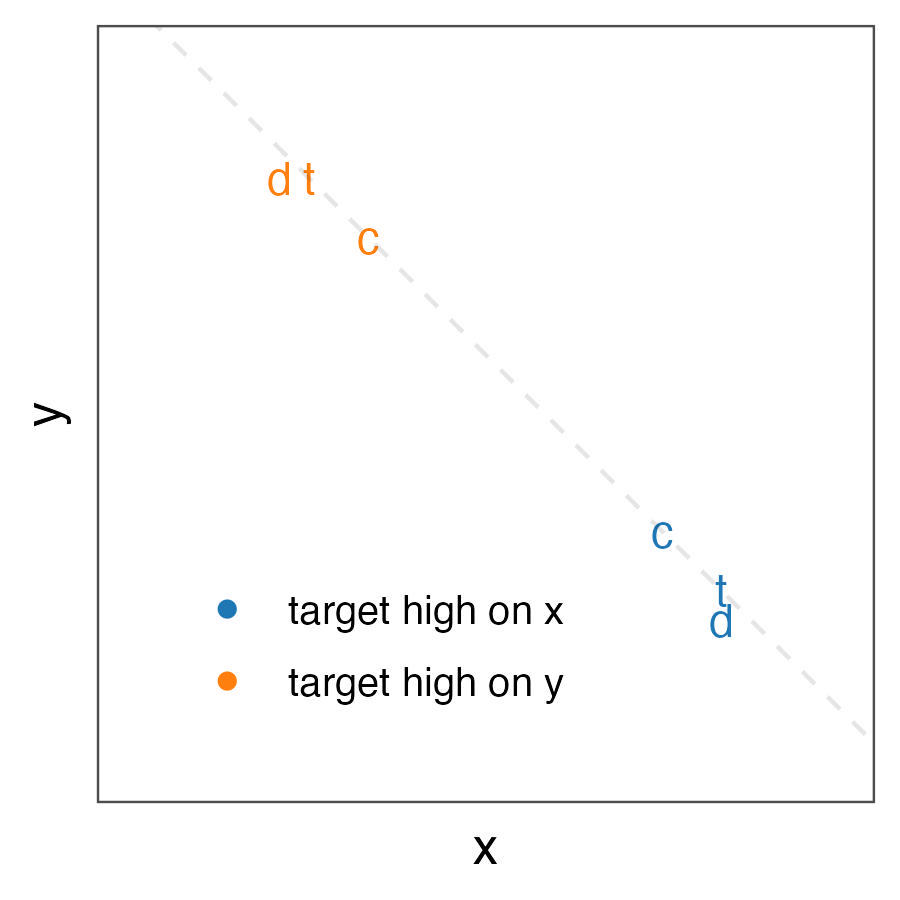
\includegraphics{figures/banerjee_stim.jpeg}
    \caption{Graphical depiction of a subset of the stimuli used in \textcite{banerjeeFactorsThatPromote2024}. Target, competitor, and decoy are labeled \textit{t}, \textit{c}, and \textit{d}, respectively. Dimensions are (generically) labeled X and Y.}. The choice sets vary based on whether the target is higher on the X or Y dimension.
    \label{fig:banerjee_stim}
\end{figure}

\textcite{banerjeeFactorsThatPromote2024}'s ompared binary to ternary choice rather than ternary to ternary choice, as in \textcite{spektorWhenGoodLooks2018b}. To do a ternary-ternary comparison, one would "flip" the target and competitor labels, such that the target is the intermediate option, the competitor is the extreme option, and the decoy is nearby the new, intermediate target. It is in one sense, quite interesting, that \textcite{banerjeeFactorsThatPromote2024} were able to generate violations of regularity in this binary to ternary comparison. However, the results are somewhat limited by the fact that the target was always more extreme than the competitor.

\textcite{banerjeeFactorsThatPromote2024} argued that their results are consistent with the "tainting hypothesis" \parencite{simonson2014vices} because the repulsion effect is strongest when the target and decoy are similar. They also argued that the decoy, may have caused participants to focus more attention on the competitor's superior dimension. For example, in the blue choice set of Figure~\ref{fig:banerjee_stim}, the decoy is quite poor on $Y$ while being equally good as the target on $X$, so participants may have focused more attention on $Y$, leading to a preference for the target. 

\textcite{banerjeeFactorsThatPromote2024}'s results are interesting and worth exploring further. The authors are also remarkably transparent about their stimulus creation procedure, in addition to posting their data online, so their stimuli were a perfect candidate for the current Experiment 4.

\section{Experiment 4}

With Experiment 4, I sought to collect ratings and choice data in a preferential choice experiment using (a subset of) \textcite{banerjeeFactorsThatPromote2024}'s stimuli. I used these data to estimate the parameters of the choice model from Chapter 2.

\subsection{Methods}

\subsubsection{Participants}
137 U.S. adults participated in the experiment. Participants were recruited from Prolific, an online platform for posting research studies, and they were paid $\$5$ for their participation. 24 participants were removed from all analyses for failing catch trials (see below), leaving a final sample size of 113. The mean age was $38.89$ ($SD=11.48$). $61$ participants identified as female, $50$ identified as male, $1$ participant identified as non-binary, and $1$ participant preferred not to say.

\subsection{Stimuli}

The stimuli were borrowed from \textcite{banerjeeFactorsThatPromote2024}'s Experiment 1. The stimuli were hypothetical consumer choice products. All stimuli varied on two attributes, each of which ranged from 0-100. The products came from four different categories: televisions, washing machines, laptops, and microwave ovens. The names of the attributes varied by category. Televisions varied on screen size and average lifespan. Washing machines varied on average lifespan and energy savings. Laptops varied on processing speed and memory (RAM). Microwave ovens varied on warranty and cooking power. 

Within the experiment, one dimension was arbitrarily designated as dimension 1 and another as dimension 2 (see below). 

\subsection{Design}

\begin{figure}
    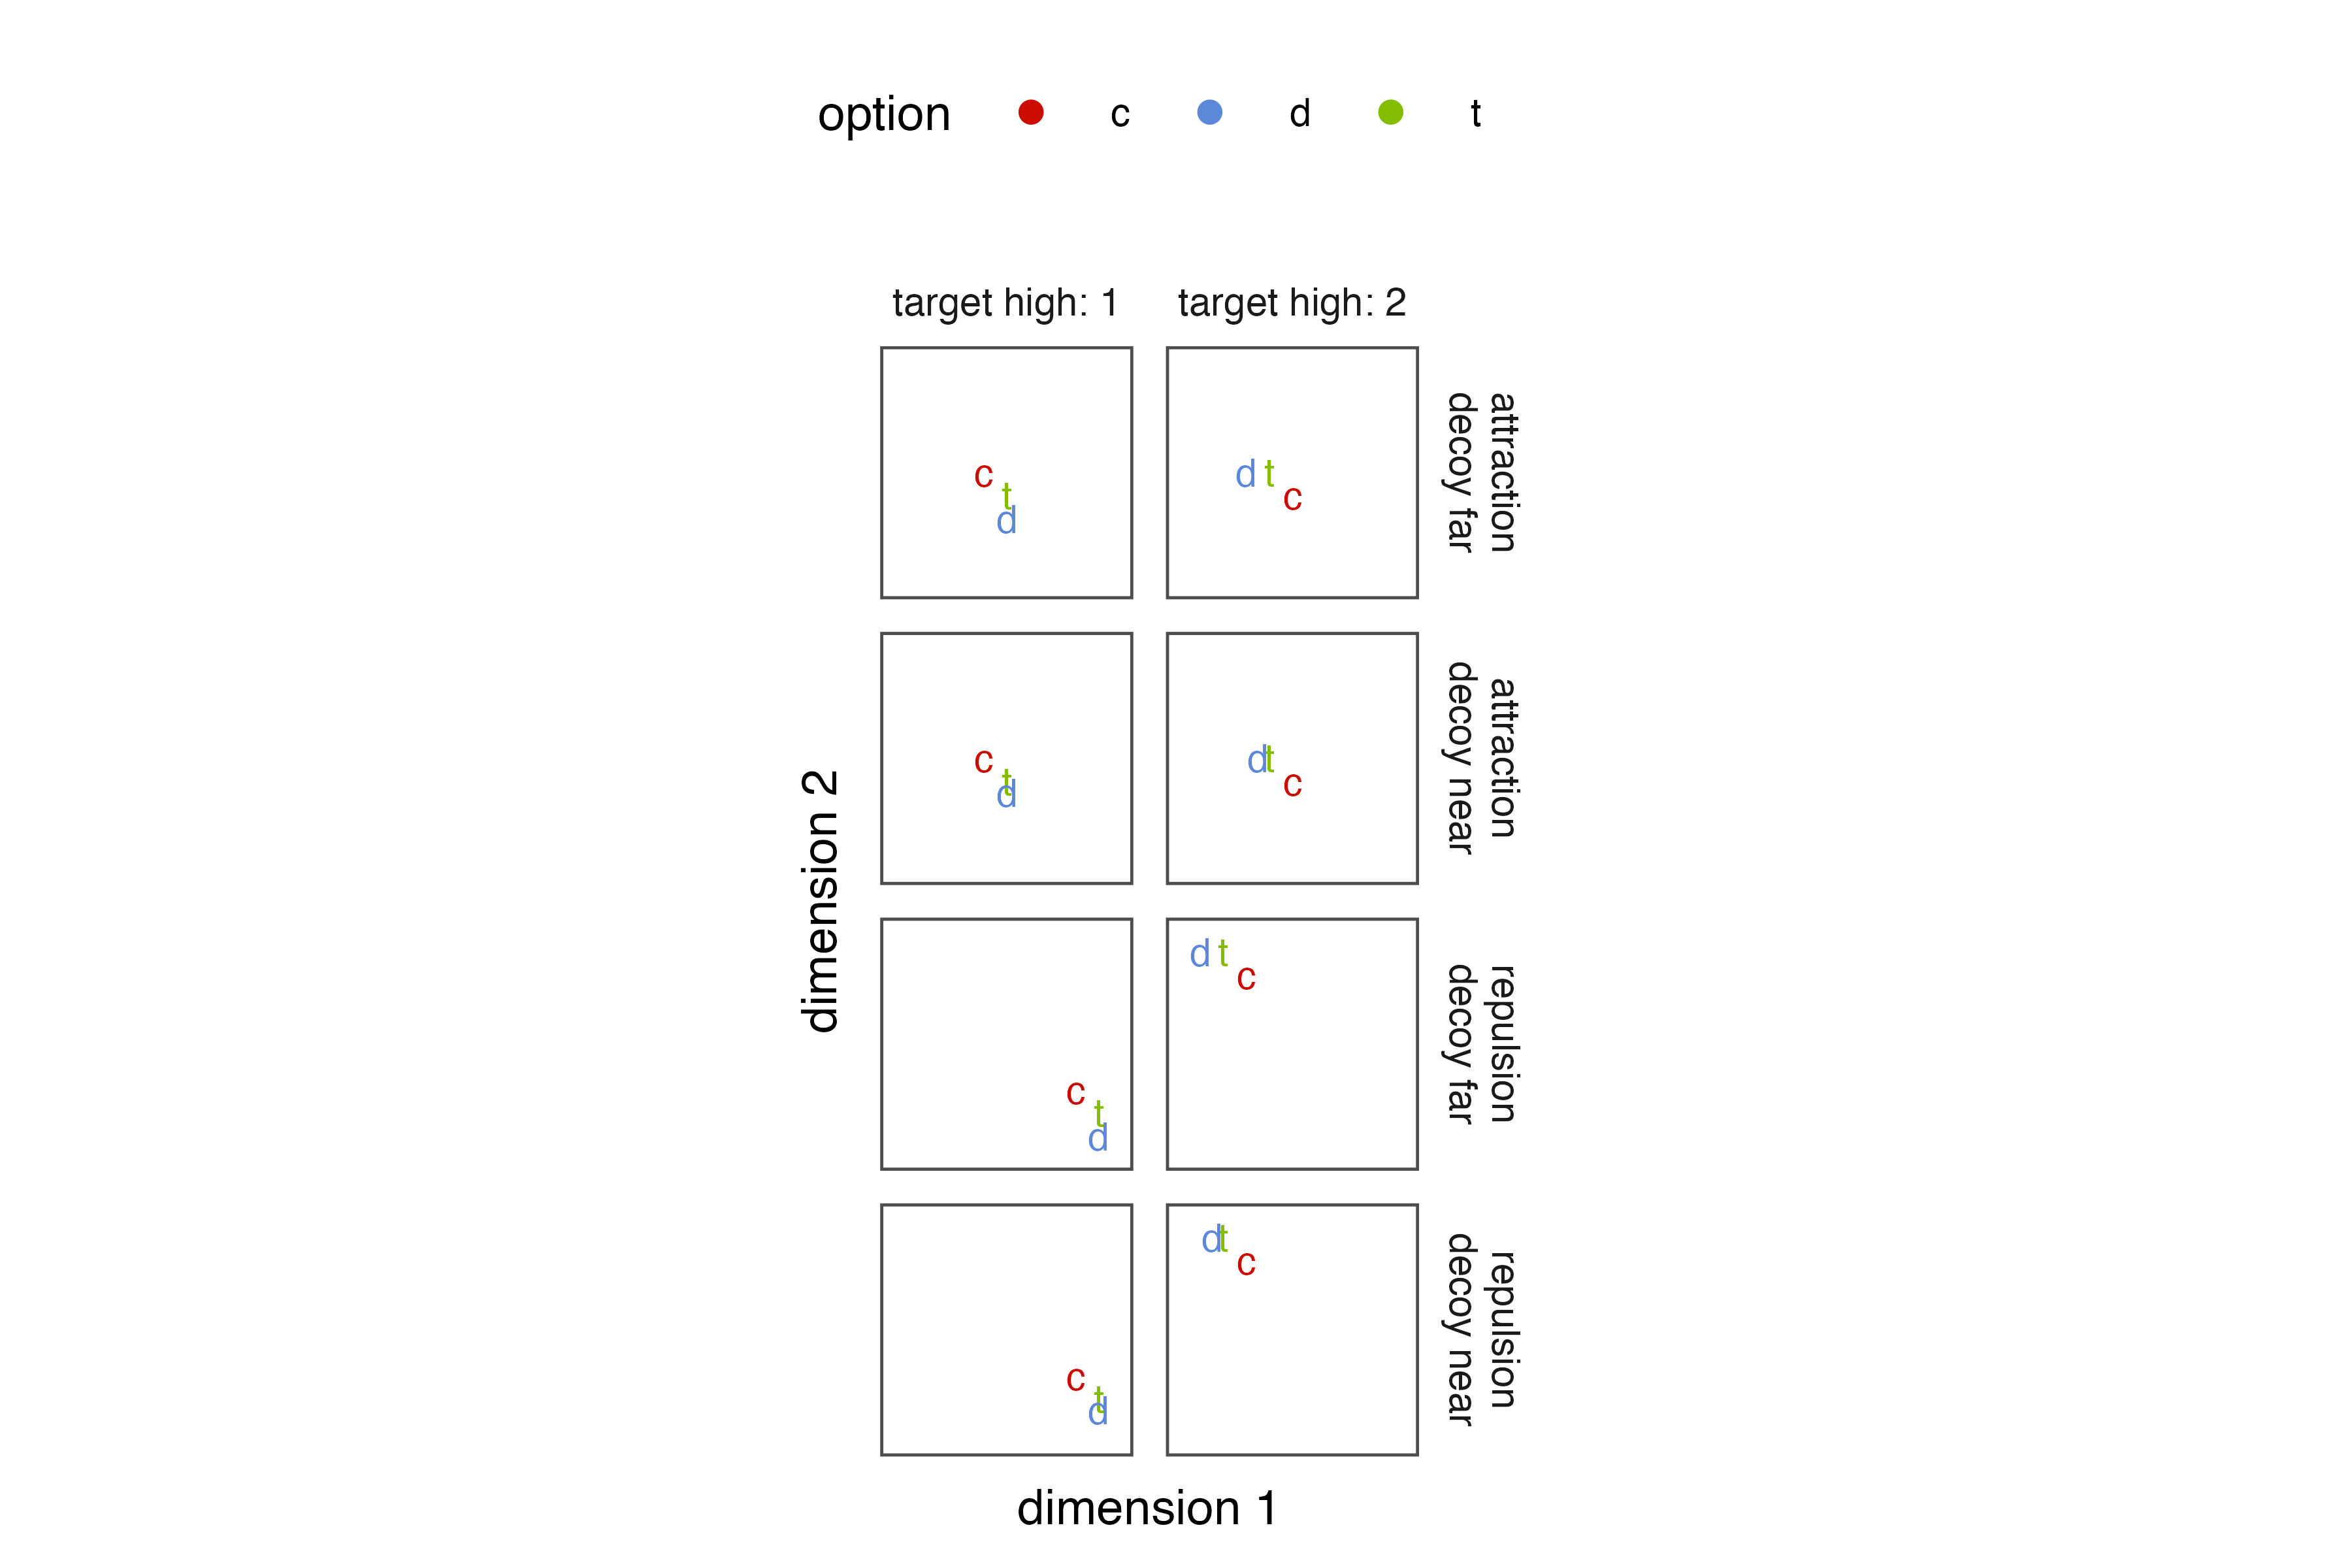
\includegraphics{figures/ce_rating_stim_for_paper.jpeg}
    \caption{Graphical depiction of a subset of the stimuli used in Experiment 4. Rows show the different choice sets designed to elicit the attraction/repulsion effect, with the label also specifying whether the decoy is near or far from the target in attribute space. The columns indicate which dimension the target is high on (1 or 2).}
    \label{fig:ce_rating_stim}
\end{figure}